\documentclass[11pt]{article}
\usepackage[utf8]{inputenc}
\usepackage{amsfonts}
\usepackage{float}
\usepackage{tikz}
\usetikzlibrary{automata, positioning, arrows}
\tikzset{
  ->,
  >=stealth',
  node distance=3cm,
  every state/.style={thick, fill=gray!10},
  initial text=$ $,
}

\setlength{\parindent}{0em}
\setlength{\parskip}{1em}

\usepackage{geometry}
\geometry{
  a4paper,
  total={170mm,257mm},
  left=20mm,
  top=20mm,
}

\title{Problem Sheet 1}
\author{Rowan Saunders}
\begin{document}

\begin{titlepage}
	\maketitle
\end{titlepage}

\section{Question 1}
\begin{enumerate}
  \item $\{a^nb^m|n\geq1, m\geq1\}$
    \begin{figure}[H]
      \centering
      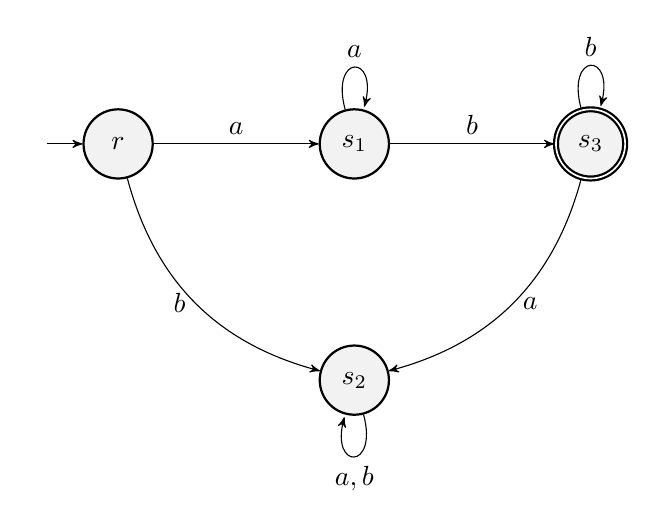
\begin{tikzpicture}
        % states
        \node[state, initial] (r) {$r$};
        \node[state, right of=r] (s1) {$s_1$};
        \node[state, accepting, right of=s1] (s3) {$s_3$};
        \node[state, below of=s1] (s2) {$s_2$};
        
        % transitions
        \draw (r) edge[above] node{$a$} (s1)
              (r) edge[bend right, left] node{$b$} (s2)
              (s1) edge[loop above] node{$a$} (s1)
              (s1) edge[above] node{$b$} (s3)
              (s3) edge[loop above] node{$b$} (s3)
              (s3) edge[bend left, right] node{$a$} (s2)
              (s2) edge[loop below] node{$a,b$} (s2);
      \end{tikzpicture}
    \end{figure}

  \item $\{a^nb^m|n$ is even OR $m$ is odd $\}$
    \begin{figure}[H]
      \centering
      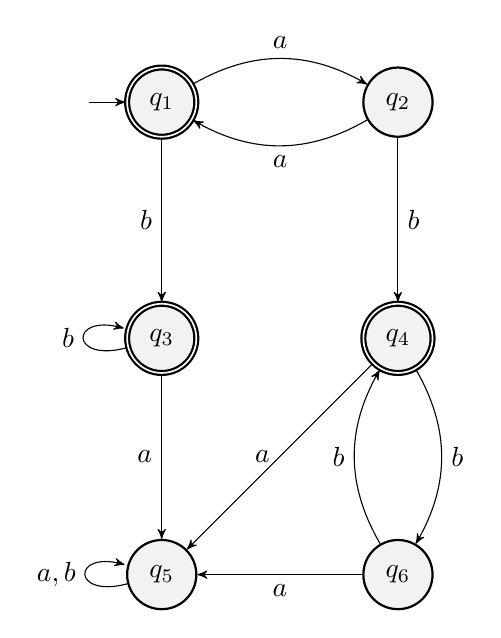
\begin{tikzpicture}
        % states
        \node[state, accepting, initial] (q1) {$q_1$};
        \node[state, right of=q1] (q2) {$q_2$};
        \node[state, accepting, below of=q1] (q3) {$q_3$};
        \node[state, accepting, right of=q3] (q4) {$q_4$};
        \node[state, below of=q3] (q5) {$q_5$};
        \node[state, right of=q5] (q6) {$q_6$};

        % transitions
        \draw (q1) edge[bend left, above] node{$a$} (q2)
              (q2) edge[bend left, below] node{$a$} (q1)
              (q1) edge[left] node{$b$} (q3)
              (q3) edge[loop left] node{$b$} (q3)
              (q3) edge[left] node{$a$} (q5)
              (q5) edge[loop left] node{$a,b$} (q5)
              (q2) edge[right] node{$b$} (q4)
              (q4) edge[left] node{$a$} (q5)
              (q4) edge[bend left, right] node{$b$} (q6)
              (q6) edge[bend left, left] node{$b$} (q4)
              (q6) edge[below] node{$a$} (q5);
        
      \end{tikzpicture}
    \end{figure}

  \item $\{w \in \{0, 1\}\ast | w = \varepsilon$ or $w$ ends in $1 \}$
    \begin{figure}[H]
      \centering
      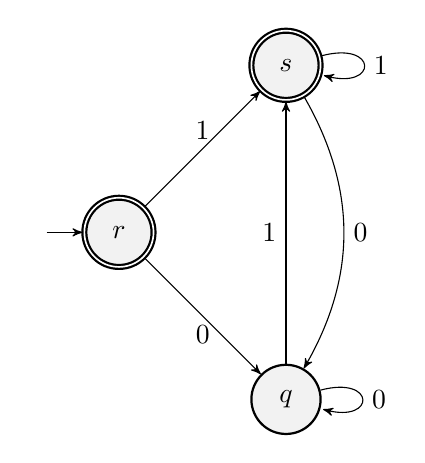
\begin{tikzpicture}
        % states
        \node[state, accepting, initial] (r) {$r$};
        \node[state, accepting, above right of=r] (s) {$s$};
        \node[state, below right of=r] (q) {$q$};
        
        % transitions
        \draw (r) edge[above] node{1} (s)
              (r) edge[below] node{0} (q)
              (s) edge[bend left, right] node{0} (q)
              (q) edge[left] node{1} (s)
              (q) edge[loop right] node{0} (q)
              (s) edge[loop right] node{1} (s);
      \end{tikzpicture}
    \end{figure}

  \item $\{w \in \{0, 1\}\ast | w $ starts and ends with $0\}$
    \begin{figure}[H]
      \centering
      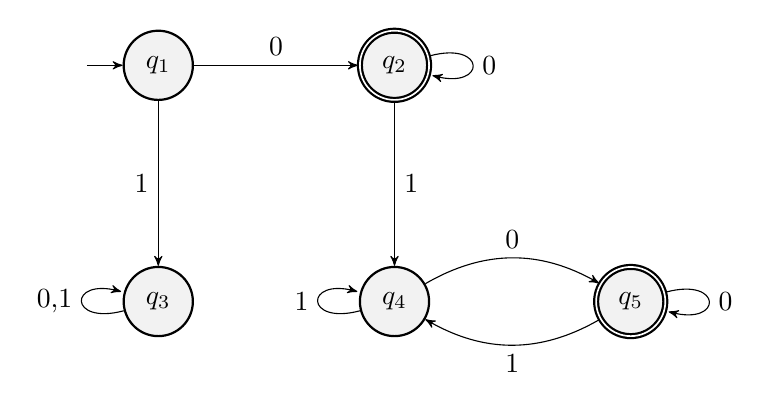
\begin{tikzpicture}
        % states
        \node[state, initial] (q1) {$q_1$};
        \node[state, accepting, right of=q1] (q2) {$q_2$};
        \node[state, below of=q1] (q3) {$q_3$};
        \node[state, right of=q3] (q4) {$q_4$};
        \node[state, accepting, right of=q4] (q5) {$q_5$};

        % transitions
        \draw (q1) edge[above] node{0} (q2)
              (q1) edge[left] node{1} (q3)
              (q3) edge[loop left] node{0,1} (q3)
              (q2) edge[loop right] node{0} (q2)
              (q2) edge[right] node{1} (q4)
              (q4) edge[loop left] node{1} (q4)
              (q4) edge[bend left, above] node{0} (q5)
              (q5) edge[bend left, below] node{1} (q4)
              (q5) edge[loop right] node{0} (q5);
        
      \end{tikzpicture}
    \end{figure}

  \item $\{w \in \{0, 1\}\ast | w $ starts and ends with the same letter$\}$
    \begin{figure}[H]
      \centering
      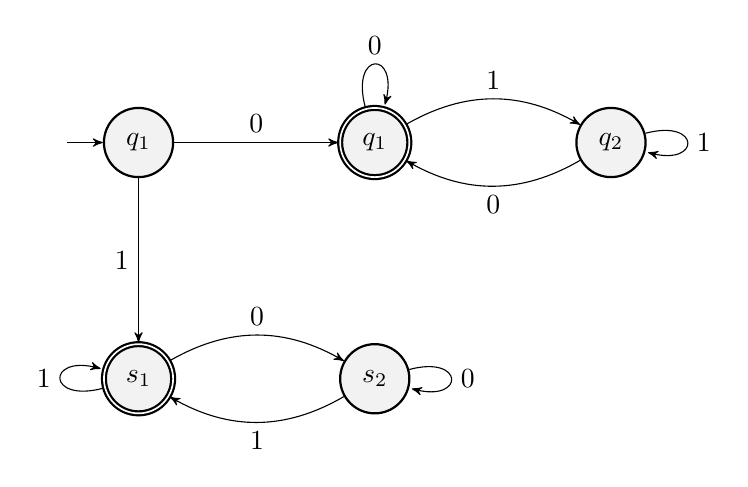
\begin{tikzpicture}
        % states
        \node[state, initial] (r) {$q_1$};
        \node[state, accepting, right of=r] (q1) {$q_1$};
        \node[state, right of=q1] (q2) {$q_2$};
        \node[state, accepting, below of=r] (s1) {$s_1$};
        \node[state, right of=s1] (s2) {$s_2$};

        % transitions
        \draw (r) edge[above] node{0} (q1)
              (r) edge[left] node{1} (s1)
              (q1) edge[loop above] node{0} (q1)
              (q1) edge[bend left, above] node{1} (q2)
              (q2) edge[bend left, below] node{0} (q1)
              (q2) edge[loop right] node{1} (q2)
              (s1) edge[loop left] node{1} (s1)
              (s1) edge[bend left, above] node{0} (s2)
              (s2) edge[bend left, below] node{1} (s1)
              (s2) edge[loop right] node{0} (s2);
        
      \end{tikzpicture}
    \end{figure}

\end{enumerate}

\section{Question 2}
From diagram 3: $\{w \in \{0, 1\}\ast | w = \varepsilon$ or $w$ ends in $1 \}$

Let
$$M = (Q,\Sigma,\delta,r,F)$$
be a finite automaton where:
\begin{center}
  $Q=\{r,s,q\}$
  
  $\Sigma=\{0,1\}$

  $\delta$ is described as:

  \begin{tabular}{ |c|c|c| }
    \hline
    $\delta$ & 0 & 1 \\
    \hline
    $r$ & $q$ & $s$ \\
    \hline
    $s$ & $q$ & $s$ \\
    \hline
    $q$ & $q$ & $s$ \\
    \hline
  \end{tabular}

  $r$ is the start state
  
  $F = \{r, q\}$
\end{center}

Alternatively $\delta$ can be written as:

$$\delta(r,0) = q$$
$$\delta(r,1) = s$$
$$\delta(q,0) = q$$
$$\delta(q,1) = s$$
$$\delta(s,0) = q$$
$$\delta(s,1) = s$$

\section{Question 3}

\begin{figure}[H]
  \centering
  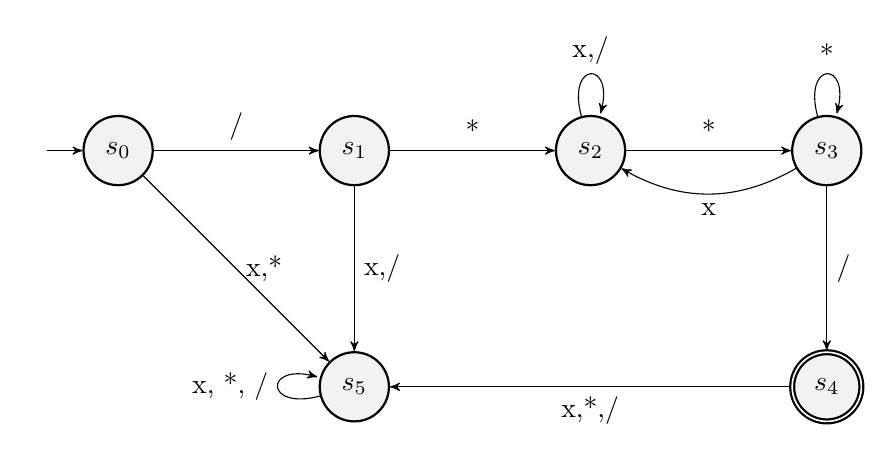
\begin{tikzpicture}
    % states
    \node[state, initial] (s0) {$s_0$};
    \node[state, right of=s0] (s1) {$s_1$};
    \node[state, right of=s1] (s2) {$s_2$};
    \node[state, right of=s2] (s3) {$s_3$};
    \node[state, accepting, below of=s3] (s4) {$s_4$};
    \node[state, below of=s1] (s5) {$s_5$};

    % transitions
    \draw (s0) edge[above] node{/} (s1)
          (s0) edge[right] node{x,*} (s5)
          (s1) edge[above] node{*} (s2)
          (s1) edge[right] node{x,/} (s5)
          (s2) edge[loop above] node{x,/} (s2)
          (s2) edge[above] node{*} (s3)
          (s3) edge[loop above] node{*} (s3)
          (s3) edge[bend left, below] node{x} (s2)
          (s3) edge[right] node{/} (s4)
          (s4) edge[below] node{x,*,/} (s5)
          (s5) edge[loop left] node{x, *, /} (s5);
    
  \end{tikzpicture}
	\caption{FSM for Java's multiline comment engine}
	\label{fig:question3}
\end{figure}

\section{Question 4}
a) $\Sigma = \{a, b\}$

Accepted:
\begin{itemize}
  \item $(b, a)$
  \item $(a, b, a)$
\end{itemize}

Rejected:
\begin{itemize}
  \item $(b, a, a, b)$
  \item $(a, a, a, b, b, a)$
\end{itemize}

$$L(M) = \{a^nba^m | n \geq 0, m \geq 0\}$$

b) $\Sigma = \{-, ), :\}$

Accepted:
\begin{itemize}
  \item $(:, -, -, ))$
  \item $(:, ))$
\end{itemize}

Rejected:
\begin{itemize}
  \item $(-, :, ))$
  \item $(:, -, -, ), ))$
\end{itemize}

$$L(M) = \{:-^n) | n \geq 0\}$$

\newpage
\section{Finite Automata Notes}
A finite automata is a 5-tuple
$ (Q, \Sigma, \delta, s_0, F) $
where $Q$ is a finite set of states, $\Sigma$ is the input alphabet, $\delta$ is the
transition function, $s_0 \in Q$ is the start state, $F \subseteq Q$ is the set of accept states.

\begin{figure}[ht]
	\centering
	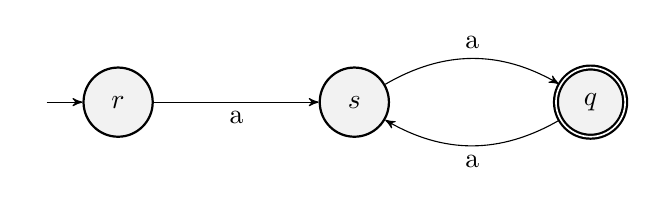
\begin{tikzpicture}
		% settings can be global or per picture
		\tikzset{
			->,
			>=stealth',
			node distance=3cm,
			every state/.style={thick, fill=gray!10},
			initial text=$ $,
		}

		% states
		\node[state, initial] (r) {$r$};
		\node[state, right of=r] (s) {$s$};
		\node[state, accepting, right of=s] (q) {$q$};

		% transitions
		\draw (r) edge[below] node{a} (s)
		(s) edge[bend left, above] node{a} (q)
		(q) edge[bend left, below] node{a} (s);

	\end{tikzpicture}
	\caption{FSM for $\{a^n | n=2m, m>0, m \in \mathbb{N} \}$}
	\label{fig:example4}
\end{figure}


For the FSM in \emph{Figure \ref{fig:example4}}:
\begin{itemize}
	\item $Q = \{r, s, q\}$
	\item $\Sigma = \{a\}$
	\item $\delta : Q \times \Sigma \to Q$
	\item $s_0 = r$
	\item $F = \{q\}$
\end{itemize}

The combination of a state and a string is a configuration.
A configuration is a pair: $(q, w) \in Q \times \Sigma\ast, (q \in Q, w \in
	\Sigma\ast)$.
With an original string of $aaaa$ the list of configurations for the FSM in
\emph{Figure \ref{fig:example4}} is:

\begin{itemize}
	\item $(r, aaaa)$
	\item $(s, aaa)$
	\item $(q, aa)$
	\item $(s, a)$
	\item $(q, \varepsilon)$
\end{itemize}

Let $(q, w)$ and $(q', w')$ be configurations, where:
$$w = aw'$$
for some letter $a \in \Sigma$, and
$$\delta(q, a) = q'$$
Then we say that $(q, w)$ yields $(q', w')$ in one step.

Therefore, $(q, aa)$ yields $(s, a)$ in one step in the example in \emph{Figure
	\ref{fig:example4}}.

For configurations $(q, w)$ and $(q', w')$ we say that $(q, w)$ yields $(q', w'$
if there is a finite sequence of configurations
$$(q_1, w_1), (q_2, w_2), ..., (q_k, w_k)$$
Such that $(q_1, w_1)=(q,w), (q_k, w_k)=(q',w')$, and
$(q_i, w_i)$ yields $(q_{i+1}, w_{i+1})$ in one step for all $i=1, 2, ..., k-1$

The sequence of configurations defined above is called a \textbf{computation}

The finite automaton $M=(Q, \Sigma, \delta, s_0, F)$ \textbf{accepts} the string
$w \in \Sigma\ast$ if $(s_0, w)$ yields $(q, \varepsilon)$ where $q \in F$.

We say that the finite automaton $M$ \textbf{recognises} the language $A$ if
$A=\{w|M \quad \mathrm{accepts} \quad w\}$.

The language \textbf{recognised by} a finite automaton $M$ is denoted $L(M)$.

The language $A$ is called regular if there exists some finite automaton $M$
such that $A = L(M)$. (i.e. a finite automaton exists that recognises it)
\end{document}
